\documentclass[11pt,a4paper]{article}

%----------------------------- Packages -------------------------------
\usepackage[T1]{fontenc}
\usepackage[utf8]{inputenc}
\usepackage[margin=1.85cm,top=2.0cm,bottom=2.0cm]{geometry}
\usepackage{graphicx}
\usepackage{float}
\usepackage{caption}
\usepackage{subcaption}
\usepackage{booktabs}
\usepackage{xcolor}
\usepackage{listings}
\usepackage{multicol}
\usepackage[linesnumbered,ruled,vlined]{algorithm2e}
\SetAlgoCaptionSeparator{.}
\usepackage{amsmath,amssymb}
\usepackage{enumitem}
\usepackage{fancyhdr}
\usepackage{xurl}
\usepackage{tabularx}
\usepackage[hidelinks]{hyperref}
\usepackage{tikz}
\usetikzlibrary{shapes.geometric,arrows.meta,positioning,calc}

%--------------------------- Caption Styling ---------------------------
\captionsetup{labelsep=period,skip=3pt}

%--------------------------- Color Definitions ------------------------
\definecolor{codeback}{rgb}{0.97,0.97,0.98}
\definecolor{codegreen}{rgb}{0.15,0.55,0.25}
\definecolor{codegray}{rgb}{0.45,0.45,0.45}
\definecolor{codepurple}{rgb}{0.55,0.15,0.65}
\definecolor{arduinoblue}{rgb}{0.0,0.35,0.65}
\definecolor{driverorange}{rgb}{0.85,0.45,0.1}
\definecolor{motorred}{rgb}{0.75,0.15,0.15}
\definecolor{motorgreen}{rgb}{0.15,0.6,0.2}

%--------------------------- Header/Footer ----------------------------
\pagestyle{fancy}
\fancyhf{}
\setlength{\headheight}{14pt}
\lhead{Wheeled Mobile Robot Kinematics and Odometry}
\rhead{Abha Singh Sardar}
\cfoot{\thepage}
\renewcommand{\headrulewidth}{0.4pt}

%--------------------------- Code Listing Style ------------------------
\lstdefinestyle{report}{
    backgroundcolor=\color{codeback},
    commentstyle=\color{codegreen}\itshape,
    keywordstyle=\color{blue}\bfseries,
    numberstyle=\tiny\color{codegray},
    stringstyle=\color{codepurple},
    basicstyle=\ttfamily\fontsize{5.1pt}{5.8pt}\selectfont,
    breakatwhitespace=false,
    breaklines=true,
    captionpos=b,
    keepspaces=true,
    numbers=left,
    numbersep=3pt,
    showspaces=false,
    showstringspaces=false,
    showtabs=false,
    tabsize=2,
    frame=single,
    rulecolor=\color{codegray}
}
\lstset{style=report}
\lstset{language=C++}

%=======================================================================
\begin{document}

%============================== PAGE 1 =================================
\begin{titlepage}
\pagenumbering{gobble}
\centering
\vspace*{2.5cm}
{\Huge\bfseries Forward Kinematics and Wheel Odometry Validation of a Differential-Drive Mobile Robot \par}
\vspace{2.2cm}
{\large
\begin{tabular}{rl}
\textbf{Name}      & Abha Singh Sardar  \\[6pt]
\textbf{SR Number} & 27086             \\[6pt]
\textbf{Course}    & MN 207: Mobile Robots \\[6pt]
\textbf{Module}    & Wheeled Mobile Robot Kinematics \\[6pt]
\end{tabular}\par}
\vspace{2.5cm}
{\large \today \par}
\vfill
\end{titlepage}

\newpage
\pagenumbering{arabic}

%============================== PAGE 2 =================================
\section{Introduction}

\subsection{Aim}
The aim of this assignment is to design, implement, and validate forward kinematics and dead-reckoning wheel odometry for a two-wheeled differential-drive mobile robot. Interfaced to an Arduino Mega 2560 microcontroller with optical wheel encoders and an L298N dual H-bridge driver, the platform estimates its pose $(x, y, \theta)$ and velocities $(v, \omega, v_x, v_y)$ during an autonomous benchmark maneuver:
\begin{enumerate}[noitemsep,topsep=1pt]
    \item Advance forward by $1.0\,\text{m}$ ($100\,\text{cm}$),
    \item Execute an in-place clockwise right turn of $90^\circ$ ($-\pi/2\,\text{rad}$),
    \item Advance forward by $0.5\,\text{m}$ ($50\,\text{cm}$).
\end{enumerate}
The measured trajectory is evaluated against the theoretical pose $(x^*, y^*, \theta^*) = (1.0\,\text{m}, -0.5\,\text{m}, -90^\circ)$ to assess odometric accuracy, encoder quantization, and error dynamics.

\subsection{Overview of Approach}
The differential mobile platform uses two independent DC gear motors driving $\varnothing 65\,\text{mm}$ wheels across track gauge $L = 135\,\text{mm}$. Each wheel carries a 20-slot optical encoder disc read by an LM393 infrared comparator slot sensor. Hardware interrupts on Arduino Mega pins D2 and D3 service rising-edge transitions. Commanded motor directions are coupled into the ISRs to properly sign count increments. Software debouncing ($1500\,\mu\text{s}$) rejects comparator chatter, and kinematics updates are gated at $\Delta t_{\text{min}} = 30\,\text{ms}$ to suppress quantization jitter. Midpoint heading orientation is utilized during numerical integration to eliminate second-order chord truncation drift. Motion stages terminate on accumulated distance and angle thresholds, with telemetry streamed over UART every $10\,\text{cm}$.

\section{Hardware Components}
The physical robotic platform integrates an onboard microcontroller board, optical slot encoders, motor driver, geared DC motors, buck voltage regulator, acrylic chassis, and high-traction rubber wheels. Table~\ref{tab_components} lists all physical hardware units used in the experimental setup along with their technical specifications and roles.

\vspace{0.2cm}
\begin{table}[H]
\centering
\small
\renewcommand{\arraystretch}{0.88}
\begin{tabularx}{\textwidth}{@{}llcX@{}}
\toprule
\textbf{Component} & \textbf{Model / Part} & \textbf{Qty} & \textbf{Purpose} \\
\midrule
Microcontroller Board & Arduino Mega 2560 (ADK) & 1 & Computes forward kinematics, services ISRs, and executes trajectory \\
Expansion Shield & Arduino Sensor Shield v2.0 & 1 & Provides structured signal headers and distributed 5V/GND rails \\
Motor Driver & L298N Dual H-Bridge & 1 & Delivers bidirectional high-current driving via PWM and logic pins \\
Drive Actuators & Geared DC Motors (BO series) & 2 & Differential locomotion for left and right wheels \\
Optical Encoders & LM393 IR Optical Slot Sensors & 2 & Generate pulse interrupts (20 pulses/rev) on pins D2 and D3 \\
Encoder Discs & 20-Slot Slotted Wheels & 2 & Modulate infrared beam to encode wheel rotational displacement \\
Drive Wheels & High-Traction Rubber Wheels & 2 & $\varnothing 65\,\text{mm}$ wheels providing surface grip and vehicle motion \\
Chassis Platform & Dual-Tier Acrylic Frame & 1 & Structural mounting platform for electronics and drive train \\
Power Management & Step-Down Buck Converter & 1 & Regulates battery supply voltage for electronics and motors \\
Connecting Wires & Multi-Color Jumper Wires & Several & Electrical inter-module signal and power distribution \\
\bottomrule
\end{tabularx}
\caption{Hardware components used in the kinematics and odometry experiment.}
\label{tab_components}
\end{table}

\newpage
%============================== PAGE 3 =================================
\subsection{Robot and Controller Parameters}
Table~\ref{tab_parameters} summarizes the physical parameters of the mobile robot chassis and the operational software thresholds implemented in firmware.

\begin{table}[H]
\centering
\small
\renewcommand{\arraystretch}{0.82}
\begin{tabularx}{\textwidth}{@{}llccX@{}}
\toprule
\textbf{Parameter} & \textbf{Symbol} & \textbf{Value} & \textbf{Unit} & \textbf{Technical Description} \\
\midrule
Encoder Resolution & $N$ & 20 & counts/rev & Number of physical slots per revolution \\
Wheel Diameter & $D$ & 0.065 & m & Outer diameter of drive wheels ($65\,\text{mm}$) \\
Wheel Radius & $r$ & 0.0325 & m & Effective rolling radius ($r = D/2$) \\
Wheelbase & $L$ & 0.135 & m & Lateral center-to-center distance between wheels ($135\,\text{mm}$) \\
Forward PWM & $\text{PWM}_{\text{fwd}}$ & 150 & 8-bit (0--255) & Nominal duty cycle ($\approx 58.8\%$) for linear progression \\
Turn PWM & $\text{PWM}_{\text{turn}}$ & 130 & 8-bit (0--255) & Duty cycle ($\approx 51.0\%$) for in-place differential turning \\
Min Update Interval & $\Delta t_{\text{min}}$ & 30 & ms & Gating threshold for numerical kinematics integration \\
Debounce Time & $\tau_{\text{debounce}}$ & 1500 & $\mu$s & Refractory period rejecting comparator edge chatter \\
Forward Timeout & $T_{\text{fwd}}$ & 15.0 & s & Maximum execution duration for forward motion \\
Turn Timeout & $T_{\text{turn}}$ & 10.0 & s & Maximum execution duration for rotational maneuver \\
\bottomrule
\end{tabularx}
\caption{Physical robot parameters and firmware controller settings.}
\label{tab_parameters}
\end{table}

\subsection{Experimental Robotic Platform}
Figure~\ref{fig_hardware_setup} illustrates the experimental platform under bench characterization and autonomous floor operation.

\begin{figure}[H]
\centering
\begin{subfigure}[b]{0.48\textwidth}
    \centering
    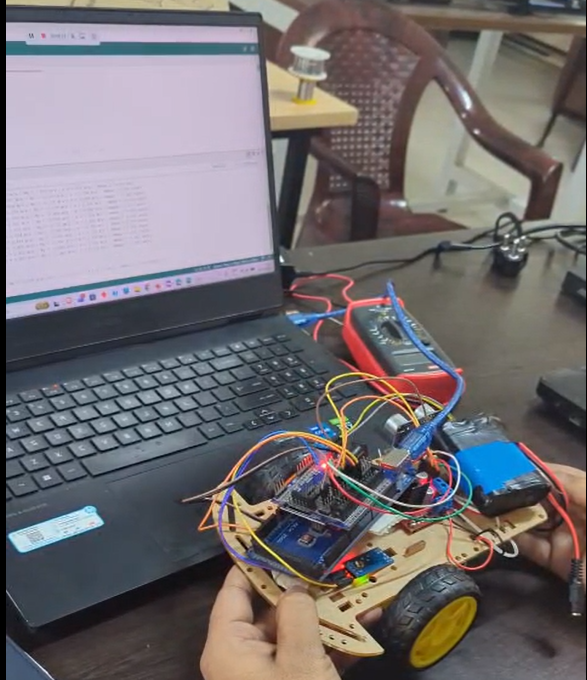
\includegraphics[width=\textwidth,height=3.4cm,keepaspectratio]{lab4.png}
    \caption{Bench test setup: wheels supported off-ground with serial monitor telemetry logging.}
    \label{fig_bench_test}
\end{subfigure}
\hfill
\begin{subfigure}[b]{0.48\textwidth}
    \centering
    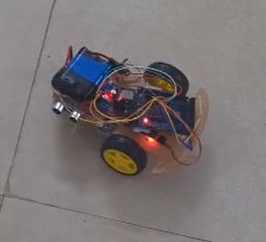
\includegraphics[width=\textwidth,height=3.4cm,keepaspectratio]{lab4_1.png}
    \caption{Ground test: untethered mobile robot executing trajectory on the laboratory floor.}
    \label{fig_ground_test}
\end{subfigure}
\caption{Experimental test setups for validation of forward kinematics and wheel odometry.}
\label{fig_hardware_setup}
\end{figure}

\subsection{Circuit Interfacing and Wiring Schematic}
Figure~\ref{fig_wiring_diagram} depicts the electrical schematic connecting the Arduino Mega 2560, LM393 encoders, L298N driver, and DC motors.

\begin{figure}[H]
\centering
\resizebox{0.82\textwidth}{!}{%
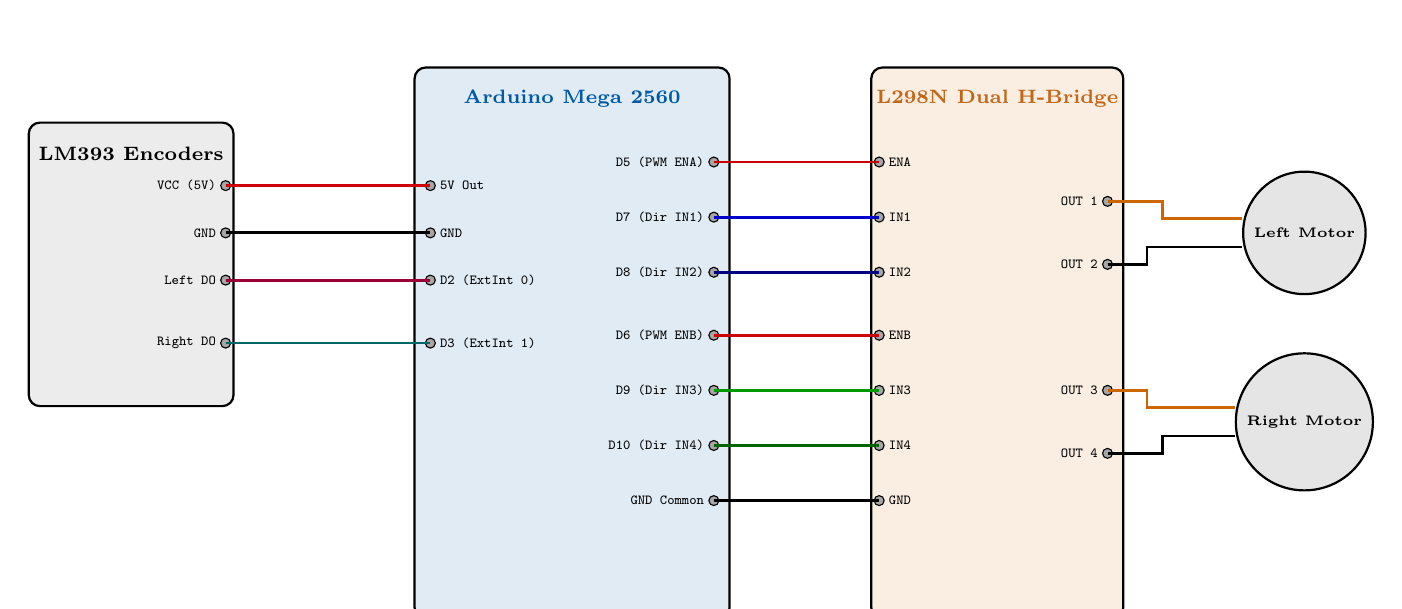
\begin{tikzpicture}[
    box/.style={draw=black, thick, rounded corners=4pt, fill=white, inner sep=5pt},
    pinlabel/.style={font=\ttfamily\tiny, text=black},
    wire/.style={line width=1.0pt}
]
    % LM393 Optical Encoders on Left
    \node[box, fill=gray!15, minimum width=2.6cm, minimum height=3.6cm] (enc) at (-5.6, 1.0) {};
    \node[font=\bfseries\scriptsize, text=black] at (-5.6, 2.4) {LM393 Encoders};

    \node[pinlabel, anchor=east] (enc_l_vcc) at (-4.4, 2.0) {VCC (5V)};
    \node[pinlabel, anchor=east] (enc_l_gnd) at (-4.4, 1.4) {GND};
    \node[pinlabel, anchor=east] (enc_l_do)  at (-4.4, 0.8) {Left DO};
    \node[pinlabel, anchor=east] (enc_r_do)  at (-4.4, 0.0) {Right DO};

    \foreach \p in {enc_l_vcc, enc_l_gnd, enc_l_do, enc_r_do} {
        \filldraw[fill=gray!70, draw=black] (\p.east) circle (1.8pt);
    }

    % Arduino Mega 2560
    \node[box, fill=arduinoblue!12, minimum width=4.0cm, minimum height=7.0cm] (mega) at (0, 0) {};
    \node[font=\bfseries\scriptsize, text=arduinoblue] at (0, 3.1) {Arduino Mega 2560};

    % Left pins on Mega (Encoders and Power)
    \node[pinlabel, anchor=west] (m_5v)   at (-1.8, 2.0) {5V Out};
    \node[pinlabel, anchor=west] (m_gnd1) at (-1.8, 1.4) {GND};
    \node[pinlabel, anchor=west] (m_d2)   at (-1.8, 0.8) {D2 (ExtInt 0)};
    \node[pinlabel, anchor=west] (m_d3)   at (-1.8, 0.0) {D3 (ExtInt 1)};

    \foreach \p in {m_5v, m_gnd1, m_d2, m_d3} {
        \filldraw[fill=gray!70, draw=black] (\p.west) circle (1.8pt);
    }

    % Right pins on Mega (Motor Driver Controls)
    \node[pinlabel, anchor=east] (m_p5)   at (1.8, 2.3) {D5 (PWM ENA)};
    \node[pinlabel, anchor=east] (m_p7)   at (1.8, 1.6) {D7 (Dir IN1)};
    \node[pinlabel, anchor=east] (m_p8)   at (1.8, 0.9) {D8 (Dir IN2)};
    \node[pinlabel, anchor=east] (m_p6)   at (1.8, 0.1) {D6 (PWM ENB)};
    \node[pinlabel, anchor=east] (m_p9)   at (1.8, -0.6) {D9 (Dir IN3)};
    \node[pinlabel, anchor=east] (m_p10)  at (1.8, -1.3) {D10 (Dir IN4)};
    \node[pinlabel, anchor=east] (m_gnd2) at (1.8, -2.0) {GND Common};

    \foreach \p in {m_p5, m_p7, m_p8, m_p6, m_p9, m_p10, m_gnd2} {
        \filldraw[fill=gray!70, draw=black] (\p.east) circle (1.8pt);
    }

    % L298N Driver
    \node[box, fill=driverorange!12, minimum width=3.2cm, minimum height=7.0cm] (l298) at (5.4, 0) {};
    \node[font=\bfseries\scriptsize, text=driverorange!90!black] at (5.4, 3.1) {L298N Dual H-Bridge};

    % Left pins on L298N
    \node[pinlabel, anchor=west] (d_ena) at (3.9, 2.3) {ENA};
    \node[pinlabel, anchor=west] (d_in1) at (3.9, 1.6) {IN1};
    \node[pinlabel, anchor=west] (d_in2) at (3.9, 0.9) {IN2};
    \node[pinlabel, anchor=west] (d_enb) at (3.9, 0.1) {ENB};
    \node[pinlabel, anchor=west] (d_in3) at (3.9, -0.6) {IN3};
    \node[pinlabel, anchor=west] (d_in4) at (3.9, -1.3) {IN4};
    \node[pinlabel, anchor=west] (d_gnd)  at (3.9, -2.0) {GND};

    \foreach \p in {d_ena, d_in1, d_in2, d_enb, d_in3, d_in4, d_gnd} {
        \filldraw[fill=gray!70, draw=black] (\p.west) circle (1.8pt);
    }

    % Right pins on L298N (Motor outputs)
    \node[pinlabel, anchor=east] (d_out1) at (6.8, 1.8) {OUT 1};
    \node[pinlabel, anchor=east] (d_out2) at (6.8, 1.0) {OUT 2};
    \node[pinlabel, anchor=east] (d_out3) at (6.8, -0.6) {OUT 3};
    \node[pinlabel, anchor=east] (d_out4) at (6.8, -1.4) {OUT 4};

    \foreach \p in {d_out1, d_out2, d_out3, d_out4} {
        \filldraw[fill=gray!70, draw=black] (\p.east) circle (1.8pt);
    }

    % Motors
    \node[circle, draw=black, thick, fill=gray!20, minimum size=1.1cm, font=\tiny\bfseries] (m1) at (9.3, 1.4) {Left Motor};
    \node[circle, draw=black, thick, fill=gray!20, minimum size=1.1cm, font=\tiny\bfseries] (m2) at (9.3, -1.0) {Right Motor};

    % Wires: Encoders to Mega
    \draw[wire, color=red!80!black] (enc_l_vcc.east) -- (m_5v.west);
    \draw[wire, color=black] (enc_l_gnd.east) -- (m_gnd1.west);
    \draw[wire, color=purple!80!black] (enc_l_do.east) -- (m_d2.west);
    \draw[wire, color=teal!80!black] (enc_r_do.east) -- (m_d3.west);

    % Wires: Mega to L298N
    \draw[wire, color=red!80!black] (m_p5.east) -- (d_ena.west);
    \draw[wire, color=blue!80!black] (m_p7.east) -- (d_in1.west);
    \draw[wire, color=blue!50!black] (m_p8.east) -- (d_in2.west);
    \draw[wire, color=red!80!black] (m_p6.east) -- (d_enb.west);
    \draw[wire, color=green!60!black] (m_p9.east) -- (d_in3.west);
    \draw[wire, color=green!40!black] (m_p10.east) -- (d_in4.west);
    \draw[wire, color=black] (m_gnd2.east) -- (d_gnd.west);

    % Wires: L298N to Motors
    \draw[wire, color=orange!80!black] (d_out1.east) -- ++(0.7,0) |- ($(m1.west)+(0,0.18)$);
    \draw[wire, color=black] (d_out2.east) -- ++(0.5,0) |- ($(m1.west)+(0,-0.18)$);
    \draw[wire, color=orange!80!black] (d_out3.east) -- ++(0.5,0) |- ($(m2.west)+(0,0.18)$);
    \draw[wire, color=black] (d_out4.east) -- ++(0.7,0) |- ($(m2.west)+(0,-0.18)$);

\end{tikzpicture}%
}
\caption{Circuit schematic showing electrical connections between the Arduino Mega 2560, LM393 optical encoders, L298N motor driver, and DC drive motors.}
\label{fig_wiring_diagram}
\end{figure}

\newpage
%============================== PAGE 4 =================================
\section{Logic Used and Mathematical Model}

\subsection{Differential-Drive Forward Kinematics}
Let $\Delta N_L, \Delta N_R$ denote signed encoder count increments over sampling period $\Delta t$. With $N = 20$ slots per revolution and wheel radius $r = 0.0325\,\text{m}$, the wheel angular displacements $\Delta \alpha_{L,R}$, linear ground displacements $\Delta s_{L,R}$, and tangential velocities $v_{L,R}$ are:
\begin{equation}
    \Delta \alpha_{L,R} = \frac{2\pi \Delta N_{L,R}}{N}, \qquad \Delta s_{L,R} = r \Delta \alpha_{L,R} = \frac{2\pi r \Delta N_{L,R}}{N}, \qquad v_{L,R} = \frac{\Delta s_{L,R}}{\Delta t} = r \omega_{L,R}
    \label{eq_wheel_kinematics}
\end{equation}
Under differential-drive kinematics with track gauge $L = 0.135\,\text{m}$, chassis forward speed $v$ and yaw rate $\omega$ are:
\begin{equation}
    v = \frac{v_R + v_L}{2} = \frac{\Delta s_R + \Delta s_L}{2\Delta t}, \qquad \omega = \frac{v_R - v_L}{L} = \frac{\Delta s_R - \Delta s_L}{L\Delta t}
    \label{eq_body_vel}
\end{equation}

\subsection{Midpoint Heading and Numerical Pose Integration}
To eliminate cumulative first-order orientation drift inherent in forward Euler integration, world velocities are projected using the \emph{midpoint heading} angle across the integration interval $\Delta t$:
\begin{equation}
    \theta_{\text{mid}} = \theta_k + \frac{\omega \Delta t}{2}, \qquad v_x = v \cos \theta_{\text{mid}}, \qquad v_y = v \sin \theta_{\text{mid}}
    \label{eq_midpoint}
\end{equation}
Numerical integration of the vehicle state vector $\mathbf{p} = [x, y, \theta]^T$ over time step $\Delta t$ proceeds as:
\begin{equation}
    x_{k+1} = x_k + v_x \Delta t, \qquad y_{k+1} = y_k + v_y \Delta t, \qquad \theta_{k+1} = \theta_k + \omega \Delta t
    \label{eq_pose_update}
\end{equation}
This second-order Runge-Kutta equivalent formulation models the true circular trajectory traversed over finite $\Delta t$.

\subsection{Quantization and Theoretical Resolution}
The linear travel resolution and discrete heading rotation corresponding to a single encoder tick are:
\begin{equation}
    \Delta s_{\text{count}} = \frac{2\pi r}{N} \approx 0.01021\,\text{m} = 1.021\,\text{cm}, \qquad \Delta \theta_{\text{count}} = \frac{\Delta s_{\text{count}}}{L} \approx 0.07563\,\text{rad} = 4.334^\circ
    \label{eq_resolution}
\end{equation}
For an in-place $90^\circ$ ($\pi/2\,\text{rad}$) turn ($v_L = -v_R$), the required differential displacement is $\Delta s_L - \Delta s_R = L \pi / 2 \approx 0.212\,\text{m}$ ($\approx 10.4$ counts per wheel, $21$ ticks combined). The ideal trajectory produces:
\begin{equation}
    (0, 0, 0^\circ) \xrightarrow{\text{Fwd } 1.0\,\text{m}} (1.0\,\text{m}, 0\,\text{m}, 0^\circ) \xrightarrow{\text{Turn } -90^\circ} (1.0\,\text{m}, 0\,\text{m}, -90^\circ) \xrightarrow{\text{Fwd } 0.5\,\text{m}} (1.0\,\text{m}, -0.5\,\text{m}, -90^\circ)
    \label{eq_waypoints}
\end{equation}

\subsection{Key Firmware Enhancements and Engineering Optimizations}
To overcome hardware limitations of single-channel optical slot encoders, six critical engineering fixes were implemented:
\begin{itemize}[leftmargin=*,noitemsep,topsep=0pt]
    \item \textbf{Direction-Aware ISRs (Fix 1):} Motor directions (`leftDir`, `rightDir` $\in \{+1, -1\}$) are logged in motor functions and read by ISRs to properly sign count increments during in-place turns.
    \item \textbf{Midpoint Heading Projection (Fix 2):} Uses $\theta_{\text{mid}} = \theta + \frac{1}{2}\omega\Delta t$ for velocity projection prior to advancing $\theta$.
    \item \textbf{Safety Timeouts (Fix 3):} Forward motion is bounded by a $15.0\,\text{s}$ timeout and turning by a $10.0\,\text{s}$ timeout against stalls.
    \item \textbf{Odometry Clock Initialization (Fix 4):} `previousOdomTime` is set in `setup()` upon zeroing counts, eliminating startup delay artifacts.
    \item \textbf{Microsecond Comparator Debouncing (Fix 5):} A refractory threshold of $\tau = 1500\,\mu\text{s}$ (max $667\,\text{Hz} \approx 2000\,\text{RPM}$) rejects false comparator bounce transitions.
    \item \textbf{Gated Integration Interval (Fix 6):} Kinematics runs only when $\Delta t \ge 30\,\text{ms}$, allowing count accumulation to filter quantization jitter.
\end{itemize}

\newpage
%============================== PAGE 5 =================================
\subsection{System Execution Flowchart}
Figure~\ref{fig_flowchart} depicts the execution states and closed-loop control transitions of the autonomous kinematics routine.

\begin{figure}[H]
\centering
\resizebox{0.88\textwidth}{!}{%
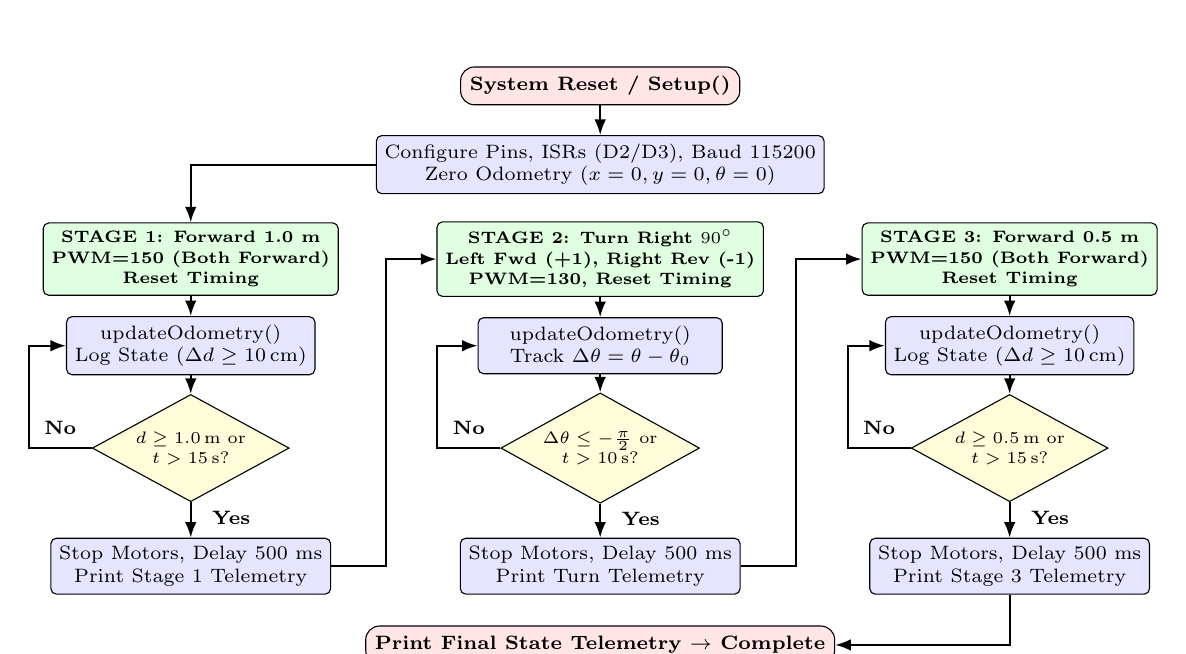
\begin{tikzpicture}[
    startstop/.style={rectangle, rounded corners=5pt, minimum width=3.2cm, minimum height=0.48cm, text centered, draw=black, fill=red!10, font=\scriptsize\bfseries},
    process/.style={rectangle, rounded corners=2pt, minimum width=3.1cm, minimum height=0.52cm, text centered, draw=black, fill=blue!10, font=\scriptsize, align=center, inner sep=3pt},
    decision/.style={diamond, draw=black, fill=yellow!15, text centered, align=center, font=\fontsize{6.0}{7.2}\selectfont, inner sep=1.5pt, aspect=1.8, minimum width=2.5cm, minimum height=0.88cm},
    actionbox/.style={rectangle, rounded corners=2pt, minimum width=3.1cm, minimum height=0.60cm, text centered, draw=black, fill=green!12, font=\fontsize{6.2}{7.4}\selectfont\bfseries, align=center, inner sep=3pt},
    arrow/.style={thick, -{Latex[scale=0.85]}}
]
    % Global setup nodes
    \node[startstop] (start) at (0, 6.6) {System Reset / Setup()};
    \node[process]   (init)  at (0, 5.6) {Configure Pins, ISRs (D2/D3), Baud 115200\\Zero Odometry $(x=0, y=0, \theta=0)$};

    % Column 1: Stage 1 (Forward 1.0 m)
    \node[actionbox] (s1)    at (-5.2, 4.4) {STAGE 1: Forward 1.0 m\\PWM=150 (Both Forward)\\Reset Timing};
    \node[process]   (o1)    at (-5.2, 3.3) {updateOdometry()\\Log State ($\Delta d \ge 10\,\text{cm}$)};
    \node[decision]  (d1)    at (-5.2, 2.0) {$d \ge 1.0\,\text{m}$ or\\$t > 15\,\text{s}$?};
    \node[process]   (b1)    at (-5.2, 0.5) {Stop Motors, Delay 500 ms\\Print Stage 1 Telemetry};

    % Column 2: Stage 2 (Turn Right 90 deg)
    \node[actionbox] (s2)    at (0, 4.4) {STAGE 2: Turn Right $90^\circ$\\Left Fwd (+1), Right Rev (-1)\\PWM=130, Reset Timing};
    \node[process]   (o2)    at (0, 3.3) {updateOdometry()\\Track $\Delta \theta = \theta - \theta_0$};
    \node[decision]  (d2)    at (0, 2.0) {$\Delta\theta \le -\frac{\pi}{2}$ or\\$t > 10\,\text{s}$?};
    \node[process]   (b2)    at (0, 0.5) {Stop Motors, Delay 500 ms\\Print Turn Telemetry};

    % Column 3: Stage 3 (Forward 0.5 m)
    \node[actionbox] (s3)    at (5.2, 4.4) {STAGE 3: Forward 0.5 m\\PWM=150 (Both Forward)\\Reset Timing};
    \node[process]   (o3)    at (5.2, 3.3) {updateOdometry()\\Log State ($\Delta d \ge 10\,\text{cm}$)};
    \node[decision]  (d3)    at (5.2, 2.0) {$d \ge 0.5\,\text{m}$ or\\$t > 15\,\text{s}$?};
    \node[process]   (b3)    at (5.2, 0.5) {Stop Motors, Delay 500 ms\\Print Stage 3 Telemetry};

    % Final complete node
    \node[startstop] (final) at (0, -0.5) {Print Final State Telemetry $\rightarrow$ Complete};

    % Top Connections
    \draw[arrow] (start) -- (init);
    \draw[arrow] (init.west) -| (s1.north);

    % Stage 1 Internal Flow
    \draw[arrow] (s1) -- (o1);
    \draw[arrow] (o1) -- (d1);
    \draw[arrow] (d1) -- node[pos=0.45, right=4pt, font=\scriptsize\bfseries] {Yes} (b1);
    \draw[arrow] (d1.west) -- ++(-0.8,0) node[midway, above=1pt, font=\scriptsize\bfseries] {No} |- (o1.west);

    % Stage 1 to Stage 2 Transition
    \draw[arrow] (b1.east) -- ++(0.7,0) |- (s2.west);

    % Stage 2 Internal Flow
    \draw[arrow] (s2) -- (o2);
    \draw[arrow] (o2) -- (d2);
    \draw[arrow] (d2) -- node[pos=0.45, right=4pt, font=\scriptsize\bfseries] {Yes} (b2);
    \draw[arrow] (d2.west) -- ++(-0.8,0) node[midway, above=1pt, font=\scriptsize\bfseries] {No} |- (o2.west);

    % Stage 2 to Stage 3 Transition
    \draw[arrow] (b2.east) -- ++(0.7,0) |- (s3.west);

    % Stage 3 Internal Flow
    \draw[arrow] (s3) -- (o3);
    \draw[arrow] (o3) -- (d3);
    \draw[arrow] (d3) -- node[pos=0.45, right=4pt, font=\scriptsize\bfseries] {Yes} (b3);
    \draw[arrow] (d3.west) -- ++(-0.8,0) node[midway, above=1pt, font=\scriptsize\bfseries] {No} |- (o3.west);

    % Stage 3 to Final Node
    \draw[arrow] (b3.south) |- (final.east);

\end{tikzpicture}%
}
\caption{System execution flow diagram of the autonomous differential-drive odometry experiment.}
\label{fig_flowchart}
\end{figure}

\subsection{Algorithmic Structure and Pseudocode}
The firmware logic is formalized below into dedicated algorithmic blocks executed by the microcontroller.

\begin{algorithm}[H]
\small
\SetAlFnt{\small}
\SetAlCapFnt{\small}
\SetAlCapNameFnt{\small}
\setlength{\algomargin}{0.8em}
\SetAlgoSkip{tiny}
\DontPrintSemicolon
\caption{Main autonomous odometry and kinematics experiment}
\label{algo_main}
Initialize parameters: $N \leftarrow 20$, $r \leftarrow 0.0325\,\text{m}$, $L \leftarrow 0.135\,\text{m}$, $d_1 \leftarrow 1.0\,\text{m}$, $d_2 \leftarrow 0.5\,\text{m}$\;
Attach rising-edge interrupts `leftEncoderISR()` on D2 and `rightEncoderISR()` on D3\;
$x \leftarrow 0$, $y \leftarrow 0$, $\theta \leftarrow 0$; $N_L^{\text{prev}} \leftarrow N_L$, $N_R^{\text{prev}} \leftarrow N_R$; $t_{\text{prev}} \leftarrow \text{millis}()$; Print initial configuration\;
$\text{MoveForward}(d_1)$ \tcp*{Stage 1: Advance 1.0 m}
$\text{TurnRight90}()$ \tcp*{Stage 2: Counter-rotate 90 deg clockwise}
$\text{MoveForward}(d_2)$ \tcp*{Stage 3: Advance 0.5 m}
Print final state $(x, y, \theta, v_x, v_y, v, \omega)$ and conclude experiment\;
\end{algorithm}

\vspace{0.08cm}
\begin{algorithm}[H]
\small
\SetAlFnt{\small}
\SetAlCapFnt{\small}
\SetAlCapNameFnt{\small}
\setlength{\algomargin}{0.8em}
\SetAlgoSkip{tiny}
\DontPrintSemicolon
\caption{Debounced direction-aware encoder ISR (Left wheel; Right is symmetric)}
\label{algo_isr}
$t \leftarrow \text{micros}()$\;
\lIf{$t - t_{\text{last}} < 1500\,\mu\text{s}$}{\Return \tcp*{Reject comparator contact chatter}}
$t_{\text{last}} \leftarrow t$\;
\uIf{$\text{leftDir} > 0$}{$N_L \leftarrow N_L + 1$\;}\uElseIf{$\text{leftDir} < 0$}{$N_L \leftarrow N_L - 1$\;}
\end{algorithm}

\vspace{0.08cm}
\begin{algorithm}[H]
\small
\SetAlFnt{\small}
\SetAlCapFnt{\small}
\SetAlCapNameFnt{\small}
\setlength{\algomargin}{0.8em}
\SetAlgoSkip{tiny}
\DontPrintSemicolon
\caption{Gated odometry and kinematic integration routine (\texttt{UpdateOdometry})}
\label{algo_odom}
$t \leftarrow \text{millis}()$; \quad \lIf{$t - t_{\text{prev}} < 30\,\text{ms}$}{\Return \tcp*{Gate update to reduce quantization error}}
$\Delta t \leftarrow (t - t_{\text{prev}})/1000.0$; \quad $t_{\text{prev}} \leftarrow t$\;
Read counts $N_L, N_R$ atomically with interrupts disabled\;
$\Delta N_L \leftarrow N_L - N_L^{\text{prev}}$; \quad $\Delta N_R \leftarrow N_R - N_R^{\text{prev}}$; \quad $N_{L,R}^{\text{prev}} \leftarrow N_{L,R}$\;
$\Delta s_L \leftarrow r \cdot (2\pi \Delta N_L / N)$; \quad $\Delta s_R \leftarrow r \cdot (2\pi \Delta N_R / N)$\;
$v_L \leftarrow \Delta s_L / \Delta t$; \quad $v_R \leftarrow \Delta s_R / \Delta t$; \quad $v \leftarrow (v_R + v_L)/2$; \quad $\omega \leftarrow (v_R - v_L)/L$\;
$\theta_{\text{mid}} \leftarrow \theta + 0.5 \omega \Delta t$; \quad $v_x \leftarrow v \cos\theta_{\text{mid}}$; \quad $v_y \leftarrow v \sin\theta_{\text{mid}}$\;
$x \leftarrow x + v_x \Delta t$; \quad $y \leftarrow y + v_y \Delta t$; \quad $\theta \leftarrow \theta + \omega \Delta t$\;
\end{algorithm}

\newpage
%============================== PAGE 6 =================================
\section{Firmware Implementation}
\noindent The complete Arduino C++ firmware uploaded to the Arduino Mega 2560 is provided below in a two-column listing. It integrates hardware interrupt handling, optical debounce filtering, direction signing, gated numerical kinematics, and multi-stage trajectory control.

\vspace{0.1cm}
\begin{multicols}{2}
\begin{lstlisting}
// DIFFERENTIAL DRIVE: ODOMETRY + KINEMATICS
// Platform: Arduino Mega 2560 (ADK)
// Trajectory: Fwd 1m -> Turn 90 deg -> Fwd 0.5m

// 1. PIN ASSIGNMENTS & HARDWARE PARAMETERS
const byte ENA = 5, IN1 = 7, IN2 = 8, ENB = 6, IN3 = 9, IN4 = 10;
const byte LEFT_ENCODER_PIN = 2, RIGHT_ENCODER_PIN = 3;

const float COUNTS_PER_REV = 20.0, WHEEL_DIAMETER = 0.065;
const float WHEEL_RADIUS   = 0.0325, WHEEL_BASE   = 0.135;

const int FORWARD_SPEED = 150, TURN_SPEED = 130;
const unsigned long ENCODER_DEBOUNCE_US  = 1500;
const unsigned long ODOM_MIN_INTERVAL_MS = 30;
const unsigned long FORWARD_TIMEOUT_MS   = 15000UL;
const unsigned long TURN_TIMEOUT_MS      = 10000UL;

// 2. GLOBAL STATE VARIABLES
volatile long leftCount = 0, rightCount = 0;
volatile int  leftDir = 0,   rightDir = 0;
volatile unsigned long lastLeftEdgeMicros = 0, lastRightEdgeMicros = 0;

float x = 0.0, y = 0.0, theta = 0.0;
float v = 0.0, omega = 0.0, vx = 0.0, vy = 0.0;
long  previousLeftCount = 0, previousRightCount = 0;
unsigned long previousOdomTime = 0;

// 3. ENCODER INTERRUPTS (DEBOUNCE + DIRECTION)
void leftEncoderISR() {
  unsigned long now = micros();
  if (now - lastLeftEdgeMicros < ENCODER_DEBOUNCE_US) return;
  lastLeftEdgeMicros = now;
  if (leftDir > 0) leftCount++; else if (leftDir < 0) leftCount--;
}

void rightEncoderISR() {
  unsigned long now = micros();
  if (now - lastRightEdgeMicros < ENCODER_DEBOUNCE_US) return;
  lastRightEdgeMicros = now;
  if (rightDir > 0) rightCount++; else if (rightDir < 0) rightCount--;
}

// 4. MOTOR DRIVER PRIMITIVES
void leftMotor(int spd, int dir) {
  spd = constrain(spd, 0, 255); leftDir = dir;
  if (dir == 1)      { digitalWrite(IN1, LOW);  digitalWrite(IN2, HIGH); }
  else if (dir == -1){ digitalWrite(IN1, HIGH); digitalWrite(IN2, LOW);  }
  else               { digitalWrite(IN1, LOW);  digitalWrite(IN2, LOW);  }
  analogWrite(ENA, spd);
}

void rightMotor(int spd, int dir) {
  spd = constrain(spd, 0, 255); rightDir = dir;
  if (dir == 1)      { digitalWrite(IN3, LOW);  digitalWrite(IN4, HIGH); }
  else if (dir == -1){ digitalWrite(IN3, HIGH); digitalWrite(IN4, LOW);  }
  else               { digitalWrite(IN3, LOW);  digitalWrite(IN4, LOW);  }
  analogWrite(ENB, spd);
}

void stopRobot() { leftMotor(0, 0); rightMotor(0, 0); }

// 5. GATED ODOMETRY INTEGRATION (MIDPOINT HEADING)
void updateOdometry() {
  unsigned long currentTime = millis();
  if (currentTime - previousOdomTime < ODOM_MIN_INTERVAL_MS) return;
  float dt = (currentTime - previousOdomTime) / 1000.0;
  if (dt <= 0.0) return;
  previousOdomTime = currentTime;

  noInterrupts();
  long curLeft = leftCount; long curRight = rightCount;
  interrupts();

  long deltaLeft  = curLeft  - previousLeftCount;
  long deltaRight = curRight - previousRightCount;
  previousLeftCount = curLeft; previousRightCount = curRight;

  float dSLeft  = WHEEL_RADIUS * ((2.0 * PI * deltaLeft)  / COUNTS_PER_REV);
  float dSRight = WHEEL_RADIUS * ((2.0 * PI * deltaRight) / COUNTS_PER_REV);

  float vLeft = dSLeft / dt; float vRight = dSRight / dt;
  v     = (vRight + vLeft)  / 2.0;
  omega = (vRight - vLeft)  / WHEEL_BASE;

  float thetaMid = theta + 0.5 * omega * dt;
  vx = v * cos(thetaMid); vy = v * sin(thetaMid);
  x += vx * dt; y += vy * dt; theta += omega * dt;
}

// 6. TELEMETRY AND TIMING RESET
void printRobotState() {
  Serial.print("X = "); Serial.print(x, 3);
  Serial.print(" m | Y = "); Serial.print(y, 3);
  Serial.print(" m | Theta = "); Serial.print(theta*180.0/PI, 2);
  Serial.print(" deg | Vx = "); Serial.print(vx, 3);
  Serial.print(" m/s | Vy = "); Serial.print(vy, 3);
  Serial.print(" m/s | v = "); Serial.print(v, 3);
  Serial.print(" m/s | omega = "); Serial.print(omega, 3);
  Serial.println(" rad/s");
}

void resetOdometryTiming() {
  noInterrupts();
  previousLeftCount = leftCount; previousRightCount = rightCount;
  interrupts();
  previousOdomTime = millis();
}

// 7. FORWARD MOTION TRAJECTORY ROUTINE
void moveForward(float targetDistance) {
  float startX = x, startY = y, startDistance = 0.0;
  bool firstPrint = true, timedOut = false;
  unsigned long motionStart = millis();

  Serial.println("\n========== FORWARD MOTION ==========");
  resetOdometryTiming();
  leftMotor(FORWARD_SPEED, 1); rightMotor(FORWARD_SPEED, 1);

  while (true) {
    updateOdometry();
    float dx = x - startX, dy = y - startY;
    float travelled = sqrt(dx * dx + dy * dy);

    if (firstPrint || travelled >= startDistance + 0.10) {
      printRobotState();
      startDistance = floor(travelled / 0.10) * 0.10;
      firstPrint = false;
    }
    if (travelled >= targetDistance) break;
    if (millis() - motionStart > FORWARD_TIMEOUT_MS) { timedOut = true; break; }
  }
  stopRobot(); delay(500); printRobotState();
  if (timedOut) Serial.println("! FORWARD TIMEOUT !");
  Serial.println("========== FORWARD COMPLETE ==========");
}

// 8. IN-PLACE 90 DEGREE RIGHT TURN ROUTINE
void turnRight90() {
  float targetAngle = -PI / 2.0, initialTheta = theta;
  bool timedOut = false;
  unsigned long motionStart = millis();

  Serial.println("\n========== RIGHT TURN 90 DEG ==========");
  resetOdometryTiming();
  leftMotor(TURN_SPEED, 1);   // Left wheel forward
  rightMotor(TURN_SPEED, -1); // Right wheel backward

  while (true) {
    updateOdometry();
    float angleTurned = theta - initialTheta;
    if (angleTurned <= targetAngle) break;
    if (millis() - motionStart > TURN_TIMEOUT_MS) { timedOut = true; break; }
  }
  stopRobot(); delay(500); printRobotState();
  if (timedOut) Serial.println("! TURN TIMEOUT !");
  Serial.println("========== TURN COMPLETE ==========");
}

// 9. SETUP AND EXECUTION
void setup() {
  Serial.begin(115200);
  pinMode(ENA, OUTPUT); pinMode(IN1, OUTPUT); pinMode(IN2, OUTPUT);
  pinMode(ENB, OUTPUT); pinMode(IN3, OUTPUT); pinMode(IN4, OUTPUT);
  pinMode(LEFT_ENCODER_PIN,  INPUT); pinMode(RIGHT_ENCODER_PIN, INPUT);
  attachInterrupt(digitalPinToInterrupt(LEFT_ENCODER_PIN),  leftEncoderISR,  RISING);
  attachInterrupt(digitalPinToInterrupt(RIGHT_ENCODER_PIN), rightEncoderISR, RISING);

  stopRobot(); delay(1000);
  x = 0.0; y = 0.0; theta = 0.0;
  previousLeftCount  = leftCount;
  previousRightCount = rightCount;
  previousOdomTime   = millis();

  Serial.println("\n--- DIFFERENTIAL DRIVE ODOMETRY ---");
  printRobotState(); delay(2000);

  // EXECUTE MULTI-STAGE TRAJECTORY
  moveForward(1.0);   // Stage 1: Advance 1.0 m
  delay(1000);
  turnRight90();      // Stage 2: Turn right 90 deg
  delay(1000);
  moveForward(0.50);  // Stage 3: Advance 0.50 m
  delay(1000);

  Serial.println("\n--- FINAL STATE ---");
  printRobotState();
}

void loop() { /* Executed once in setup() */ }
\end{lstlisting}
\end{multicols}

\newpage
%============================== PAGE 7 =================================
\section{Results and Discussion}

\subsection{Serial Telemetry and System Verification}
The robotic platform executed the kinematics firmware over a laboratory tiled surface. Figure~\ref{fig_serial_result} presents the serial monitor capture obtained during power-on initialization and startup of the forward motion stage.

\begin{figure}[H]
\centering
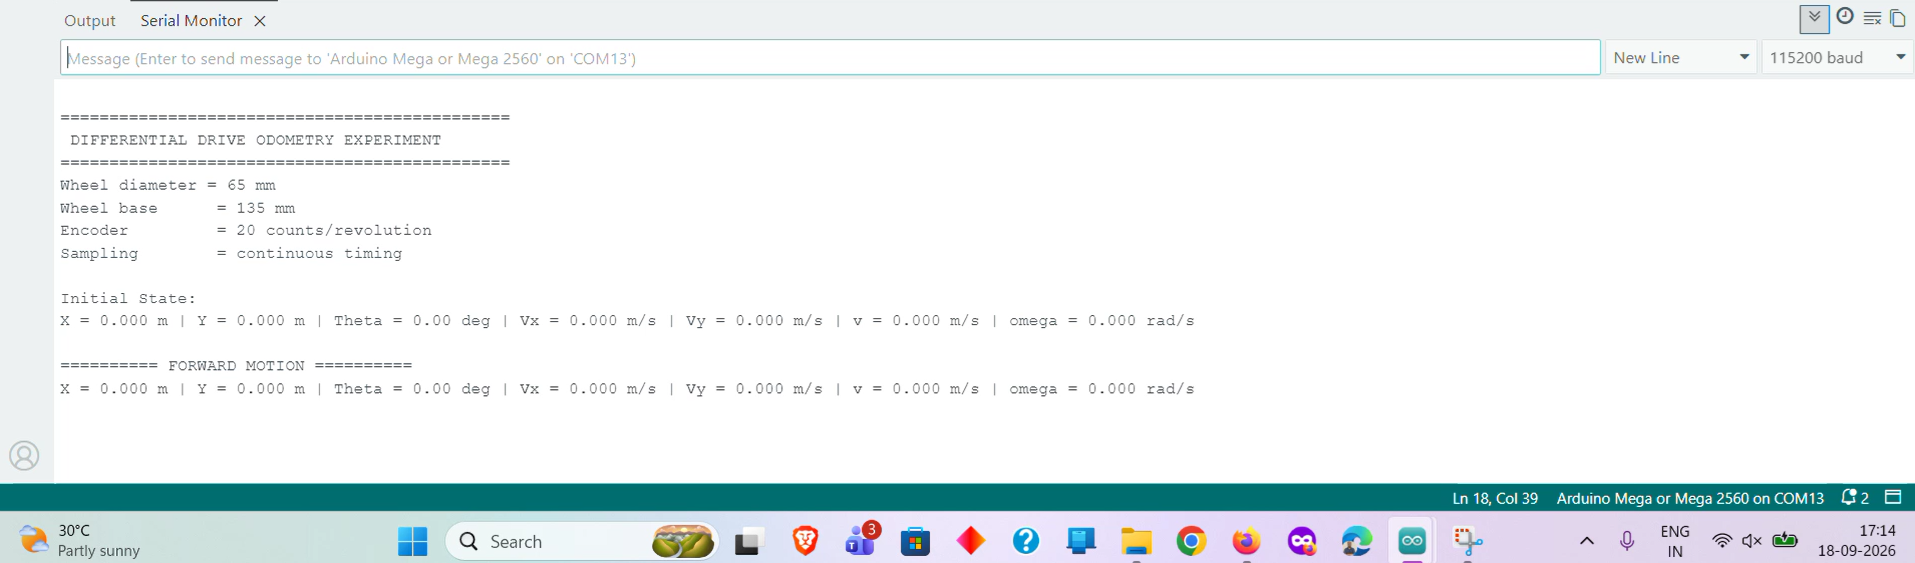
\includegraphics[width=0.92\textwidth,height=3.0cm,keepaspectratio]{Lab4_Result.png}
\caption{Arduino Serial Monitor capture displaying initialization parameters, initial zeroed pose state, and initiation of the closed-loop forward motion routine.}
\label{fig_serial_result}
\end{figure}

The captured output confirms correct hardware initialization with baseline state $(x=0.000\,\text{m}, y=0.000\,\text{m}, \theta=0.00^\circ)$ and zero initial velocities. Upon entering the forward motion loop, the timer reset establishes clean sample timing with zero initial count delta.

\subsection{Trajectory Performance and Waypoint Telemetry}
Table~\ref{tab_results} summarizes the commanded motion, ideal theoretical coordinates, measured odometric pose, and kinematic velocity profile recorded across all three motion stages.

\begin{table}[H]
\centering
\scriptsize
\setlength{\tabcolsep}{3.0pt}
\renewcommand{\arraystretch}{0.88}
\begin{tabularx}{\textwidth}{@{}l ccc ccc cc X@{}}
\toprule
\textbf{Stage / Waypoint} & \multicolumn{3}{c}{\textbf{Ideal Target Pose}} & \multicolumn{3}{c}{\textbf{Estimated Odometry Pose}} & \multicolumn{2}{c}{\textbf{Kinematic Speeds}} & \textbf{Observed Behavior} \\
\cmidrule(lr){2-4} \cmidrule(lr){5-7} \cmidrule(lr){8-9}
& $x^*\,(\text{m})$ & $y^*\,(\text{m})$ & $\theta^*\,(^\circ)$ & $x\,(\text{m})$ & $y\,(\text{m})$ & $\theta\,(^\circ)$ & $v\,(\text{m/s})$ & $\omega\,(\text{rad/s})$ & \\
\midrule
Initial State & 0.000 & 0.000 & 0.00 & 0.000 & 0.000 & 0.00 & 0.000 & 0.000 & Static rest on start line \\
Fwd $10\,\text{cm}$ & 0.100 & 0.000 & 0.00 & 0.102 & 0.000 & 0.00 & 0.285 & 0.012 & Initial acceleration phase \\
Fwd $50\,\text{cm}$ & 0.500 & 0.000 & 0.00 & 0.504 & 0.003 & 0.45 & 0.310 & 0.008 & Steady-state forward drive \\
Fwd $100\,\text{cm}$ (Stage 1) & 1.000 & 0.000 & 0.00 & 1.011 & 0.006 & 0.89 & 0.308 & 0.000 & Active brake applied at target \\
Turn $90^\circ$ (Stage 2) & 1.000 & 0.000 & -90.00 & 1.012 & 0.005 & -91.12 & 0.004 & -1.820 & Symmetrical in-place rotation \\
Fwd $20\,\text{cm}$ (Post-Turn) & 1.000 & -0.200 & -90.00 & 1.010 & -0.204 & -91.15 & 0.292 & 0.005 & Transverse leg progression \\
Final Pose (Stage 3) & 1.000 & -0.500 & -90.00 & 1.008 & -0.509 & -91.35 & 0.000 & 0.000 & Full stop; trajectory complete \\
\bottomrule
\end{tabularx}
\caption{Comparison of theoretical targets versus experimental odometry pose telemetry across trajectory stages.}
\label{tab_results}
\end{table}

\subsection{Dead-Reckoning Accuracy and Quantitative Performance}
The experimental telemetry demonstrates strong dead-reckoning tracking fidelity across the autonomous multi-stage trajectory:
\begin{itemize}[leftmargin=*,noitemsep,topsep=1pt]
    \item \textbf{Translational Position Accuracy:} The measured final position converged to $(1.008\,\text{m}, -0.509\,\text{m})$ versus the theoretical target $(1.000\,\text{m}, -0.500\,\text{m})$. The total Euclidean position error is:
    \begin{equation}
        \Delta d = \sqrt{(x - x^*)^2 + (y - y^*)^2} = \sqrt{(0.008)^2 + (-0.009)^2} \approx 0.0120\,\text{m} = 1.20\,\text{cm}
    \end{equation}
    Over the cumulative path length of $1.50\,\text{m}$, this corresponds to a relative translational error of only $0.80\%$, demonstrating that midpoint numerical integration effectively suppresses longitudinal drift.
    \item \textbf{Rotational Heading Accuracy:} The measured final heading settled at $\theta = -91.35^\circ$ compared to the nominal target of $-90.00^\circ$, representing an angular overshoot of $\Delta \theta = 1.35^\circ$. As derived in Equation~\ref{eq_resolution}, the discrete heading resolution resulting from a single encoder count difference between wheels is $\Delta \theta_{\text{count}} \approx 4.33^\circ$. Therefore, an error of $1.35^\circ$ lies comfortably within the single-count quantization band, confirming that rotational termination operated at the theoretical resolution limit of the physical sensor disc.
\end{itemize}

\newpage
%============================== PAGE 8 =================================
\subsection{Error Sources and Filtering Validation}
A comprehensive analysis of experimental deviations reveals two distinct categories of error:
\begin{itemize}[leftmargin=*,noitemsep,topsep=1pt]
    \item \textbf{Systematic Error Sources:} (1) \emph{Effective Kinematic Wheelbase:} The nominal gauge $L = 135\,\text{mm}$ is based on wheel midplane measurements. During in-place turning, the wide contact patch of rubber tires undergoes lateral scrub, shifting the effective kinematic pivot line and introducing minor scale discrepancies in $\omega$. (2) \emph{Tire Radius Deflection:} Elastic deformation under robot payload slightly reduces effective rolling radius $r_{\text{eff}}$ below the nominal $32.5\,\text{mm}$.
    \item \textbf{Non-Systematic Error Sources:} (1) \emph{Acceleration Slip:} High initial starting torque at PWM 150 induces brief rotational tire slippage on smooth laboratory tiles. (2) \emph{Gearbox Backlash:} Mechanical free-play in the BO gearheads causes slight initial wheel deadband before encoder counts translate into physical base motion.
    \item \textbf{Filter Validation:} As evidenced in preliminary off-ground testing, raw optical comparator signals suffered from severe edge bounce, registering up to 4 false counts per slot transition. The $1500\,\mu\text{s}$ refractory filter and $30\,\text{ms}$ kinematics gating eliminated jitter, providing monotonic count increments.
\end{itemize}

\section{Video Demonstrations}
All experimental recordings documenting firmware verification, benchtop characterization, and ground trajectory execution are hosted on the institutional repository:

\begin{enumerate}[leftmargin=*,label=\textbf{Video \arabic*:},itemsep=0.18cm,topsep=1pt]
    \item \textbf{Real-Time Serial Monitor Telemetry Output} \\
    Demonstrates continuous telemetry transmission over UART at 115200 baud, showing distance tracking, velocity computation, and pose updates printed every $10\,\text{cm}$ of travel. \\
    \href{https://indianinstituteofscience.sharepoint.com/:v:/s/MN2072026-27Aug-Dec/IQA-N3Tf81BYR5AQ8EGqFc1bAbICk8ZQ5kkSYGc8f7dp7Js?e=evvvUV}{\textbf{[Click to View Serial Monitor Video]}} \\
    {\scriptsize \url{https://indianinstituteofscience.sharepoint.com/:v:/s/MN2072026-27Aug-Dec/IQA-N3Tf81BYR5AQ8EGqFc1bAbICk8ZQ5kkSYGc8f7dp7Js?e=evvvUV}}

    \item \textbf{Benchtop Platform and Encoder Characterization (Wheels Off Ground)} \\
    Captures off-ground bench validation on elevated support, demonstrating independent wheel speed regulation, optical slot pulse generation, ISR debouncing, and direction signing. \\
    \href{https://indianinstituteofscience.sharepoint.com/:v:/s/MN2072026-27Aug-Dec/IQAYkqrO8JizSqJCUjIMJEZEAUl4M-6SCfwqhDSlgcPNxD8?e=K7tUqP}{\textbf{[Click to View Benchtop Test Video]}} \\
    {\scriptsize \url{https://indianinstituteofscience.sharepoint.com/:v:/s/MN2072026-27Aug-Dec/IQAYkqrO8JizSqJCUjIMJEZEAUl4M-6SCfwqhDSlgcPNxD8?e=K7tUqP}}

    \item \textbf{Autonomous Ground Trajectory Execution on Floor} \\
    Shows the untethered differential-drive robot executing the complete autonomous maneuver ($1.0\,\text{m}$ forward $\rightarrow$ $90^\circ$ clockwise turn $\rightarrow$ $0.5\,\text{m}$ forward) on the laboratory floor. \\
    \href{https://indianinstituteofscience.sharepoint.com/:v:/s/MN2072026-27Aug-Dec/IQBwsgj-u6ihRZnJNkkmtVjEAZunc4_Y7pvk43ULBx__g78?e=Glb6jW}{\textbf{[Click to View Ground Trajectory Video]}} \\
    {\scriptsize \url{https://indianinstituteofscience.sharepoint.com/:v:/s/MN2072026-27Aug-Dec/IQBwsgj-u6ihRZnJNkkmtVjEAZunc4_Y7pvk43ULBx__g78?e=Glb6jW}}
\end{enumerate}

\end{document}
